% Chapter Template

\chapter{Methodology}

\label{Methodology}

\section{Pose}

The methodology throughout this section is dependent on pose information output from models that were described in section \ref{sec:pose-detection}. These pose models output several outputs used by similar models such as joint heatmaps, however the main focus of this paper is the pure positions of the joints. These joints can be connected by lines to form "bones" which are then all connected together to form a "skeleton". This skeleton is shown in figure \ref{fig:pose}, where each of the joints are connected to form a human-like figure that can easily be created form the x \& y coordinates of the joints.

\begin{figure}[h]
	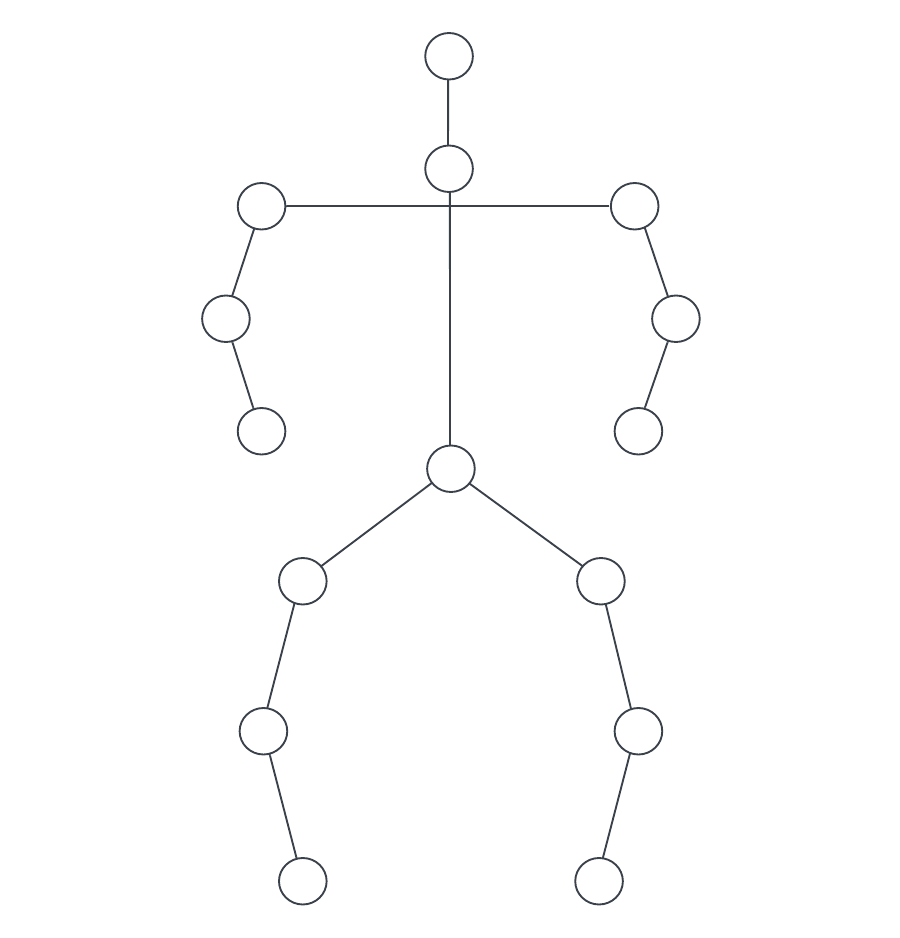
\includegraphics[width=5cm]{pose}
	\centering
	\caption{Example of how joints are connected through bones in pose representations.}
	\label{fig:pose}
\end{figure}

Using the JHMDB dataset, we simply take the existing pose implementation, the representation and indexes being shown in figure \ref{fig:JHMDB}, where there are 15 total joints. Specifically in this thesis, we are concerned with bone-joint-bone connections, effectively representing the angle of the middle joint and how the bones around it move.

\subsection{Joint Angles}

The core of how the new representation will represent actions and movement have to do with the angle between two bones at any one given joint.

\begin{figure}[h]
	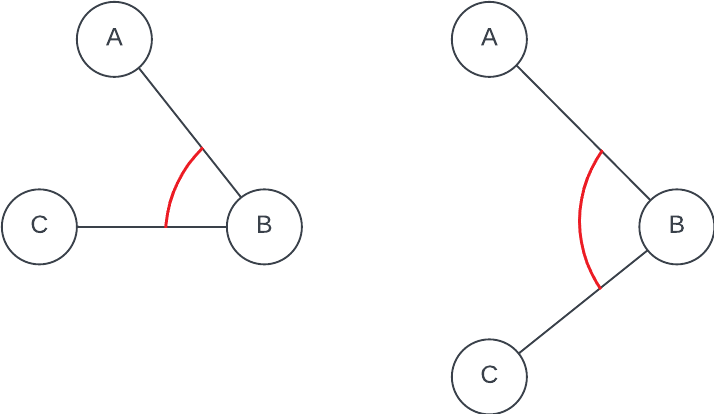
\includegraphics[width=5cm]{JointAngles}
	\centering
	\caption{}
	\label{fig:joint-angles}
\end{figure}

The first step in calculating the directional angle between the two vectors is to center them at the origin. Throughout this chapter, we will be referring to these two vectors as $a$ and $b$. Which in figure \ref{fig:joint-angles}, "$a$" would be denoting the vector $B \rightarrow A$ and "$b$" the vector $B \rightarrow C$. This origin centering is simple and is done by the following equation \ref{eqn:angle-centering}, with each point representation as it was in figure \ref{fig:joint-angles} using the $B \rightarrow A$ bone as an example.

\begin{equation}
	\label{eqn:angle-centering}
	\centering
	VectorA(x,y) = (A.x - B.x, A.y - B.y)
\end{equation}

After processing both bones through this equation, it produces two vectors beginning at the origin. The goal then becomes calculating the angle between two of these vectors. This can be easily done by leveraging arctan. Calculating the angle of a given vector '$a$' to the x-axis is simply done by using $\arctan(a.y/a.x)$. Once we have the angle of this vector to the x-axis, we can convert it to a positive value to ensure that the angle is being measured from a clockwise direction. Afterwards, we simply take the difference of the two vectors to determine the clockwise directional angle between two given vectors as denoted in equation \ref{eqn:angle-calculation}.

\begin{equation}
	\label{eqn:angle-calculation}
	\centering
	\arctan(a.y/a.x) - \arctan(b.y/b.x)
\end{equation}

The angle is calculated in a particular direction because if it were simply to be calculated agnostic of direction, it would be impossible to determine what angle a joint moves if it were to cross the $180^\circ$ boundary. Table \ref{tab:directed-angle-example} demonstrates this issue, where a $180^\circ$ rotation is observed from one right angle to another, but if non-directional angle is used, no change is represented.

\begin{table}[h]
	\centering
	\begin{tabular}{||c c c c||} 
		\hline
		\textbf{a(x,y)} & \textbf{b(x,y)} & \textbf{Directional Diff} & \textbf{Non-Directional Diff} \\ [0.5ex] 
		\hline\hline
		$(1,0)$ & $(0,1)$ & $90^\circ$ & $90^\circ$ \\
		\hline
		$(1,0)$ & $(0,-1)$ & $270^\circ$ & $90^\circ$ \\
		\hline
	\end{tabular}
	\label{tab:directed-angle-example}
	\caption{Example of how non-directional angle can result in incorrect rotation changes from one frame to another.}
\end{table}

The resulting method means that some angles will be measured from the "outside" of the person and some will be measured from the "inside" as shown in figure \ref{fig:pose-joint-angles}. In practice, this does not have a large effect on the representation as the primary factor in this method is the change of an angle from one frame to another which is indifferent to how the angle is measured as long as the distance is consistent.

\begin{figure}[h]
	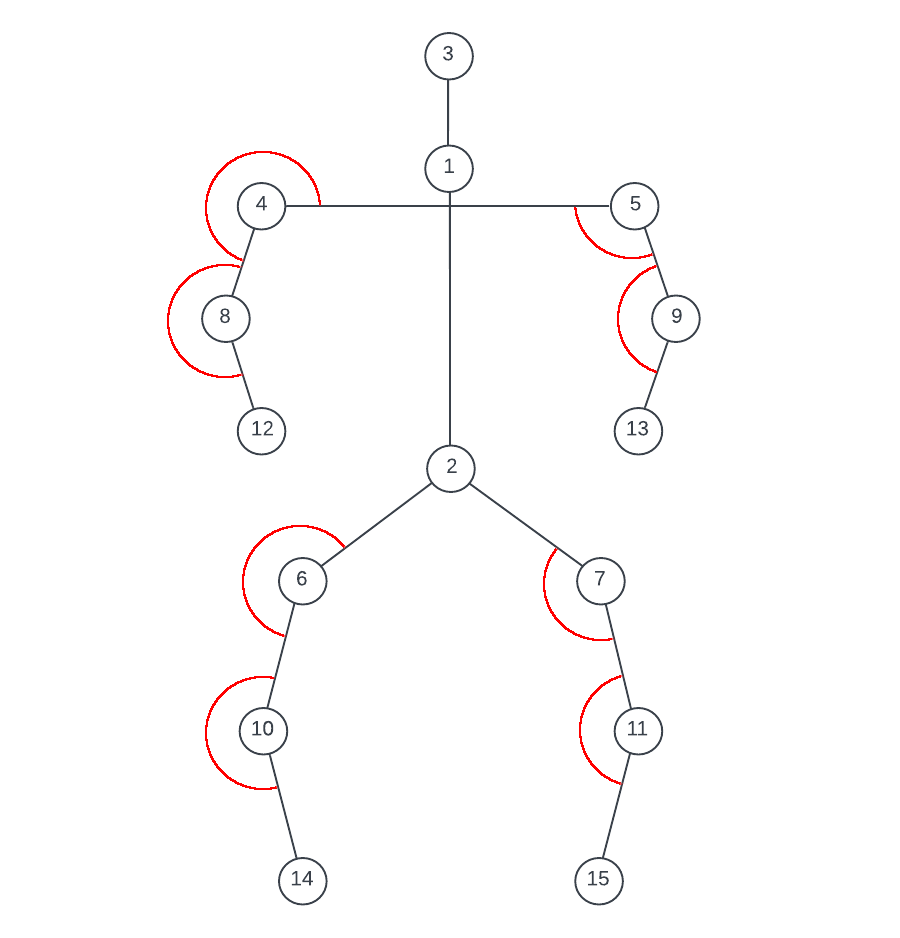
\includegraphics[width=5cm]{PoseJointAngles}
	\centering
	\caption{}
	\label{fig:pose-joint-angles}
\end{figure}

\subsection{Joint Velocities}

Once the joint angles for each frame have been extracted, the next step before implementation into our representation is to determine the change of a joint angle from one frame to another to determine the "velocity" of said joint angle. Generally this is simply done by calculating $angle(b) - angle(a)$, however there is one exception where the angle change crosses over the positive x-axis. This would be an example such as the difference between $a = 5$ and $b = 350$. The correct description would be that the angle moved $-15^\circ$, however using that simple calculation would mean that the model would interpret this as a $345^\circ$ change. This is most likely incorrect, as the more likely scenario is that the person moved $-15^\circ$ rather than almost a complete rotation in the other direction. So we add logic such that if the difference between two angles is greater than $180^\circ$ or lower than $-180^\circ$, the most likely scenario is that it moved in the opposite direction for a shorter distance. So a change such as $270^\circ$ would become $-90^\circ$ and similarly a change of $-270^\circ$ would become $90^\circ$.

\section{Novel Intermediate Representation}

\begin{figure}[h]
	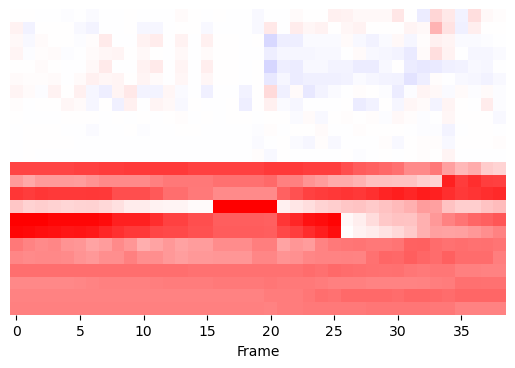
\includegraphics[width=8cm]{IntermediateStacked}
	\centering
	\caption{}
	\label{fig:intermediate-stacked}
\end{figure}

\subsection{Temporal Adjustments}

\begin{figure}
	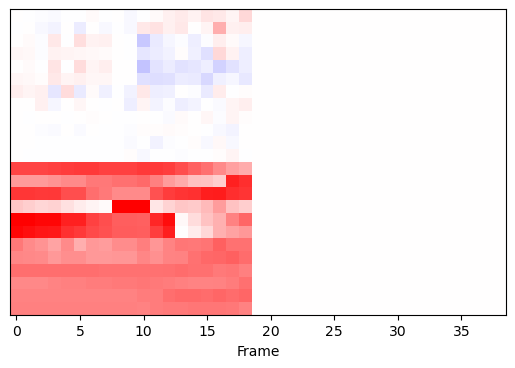
\includegraphics[width=8cm]{IntermediateSkip1}
	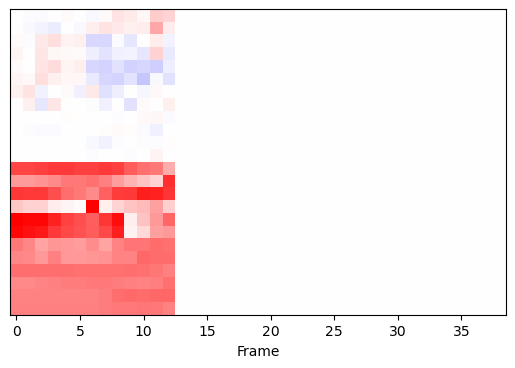
\includegraphics[width=8cm]{IntermediateSkip2}
	\centering
	\caption{}
	\label{fig:intermediate-stacked-skip}
\end{figure}

\subsection{Model Architecture}